\section{Work-in-progress: \\ private \knn{} queries}

	\begin{frame}[label={frame:knn}]

		\frametitle{General idea}

		\begin{itemize}
			\item<1->
				Model: \alert{snapshot}, query type: \alert{\knn{}} in arbitrary dimensions

			\item<2->
				Nearest-neighbor search needs definitions of \emph{object} and \emph{distance} \\
				\begin{small}
					\indent{} Object could be 2D/3D location, or a document embedding (high-dimensional vector) \\
					\indent{} Distance can be $\text{L}_\text{p}$ (usually, Euclidean, $p = 2$) or inner (dot) product
				\end{small}

			\item<3->
				Applications range from similarity search to geographical search \\
				\begin{small}
					\indent{} Object on a map is a 2D vector, query is to find $k$ nearest locations \\
					\indent{} Document is a vector of words/features/topics, query is to find $k$ most similar documents
				\end{small}

			\item<4->
				Our approach is to apply a \emph{property-preserving encryption} on objects \\
				\begin{small}
					\indent{} Query protocol is then similar to OPE/ORE \\
					\indent{} Existing nearest-neighbor search algorithms then work naturally
				\end{small}

			\item<5->
				\textbf{Study how accuracy of search and efficiency of attacks drop with higher security}

		\end{itemize}

	\end{frame}

	\begin{frame}{Distance Comparison Preserving Encryption}

		\[
			\forall x, y, x \in \mathbb{X} : \algo{Dist}{x, y} < \algo{Dist}{x, z} - \beta \implies \algo{Dist}{f(x), f(y)} < \algo{Dist}{f(x), f(z)}
		\]

		\begin{figure}[h]
			\centering
			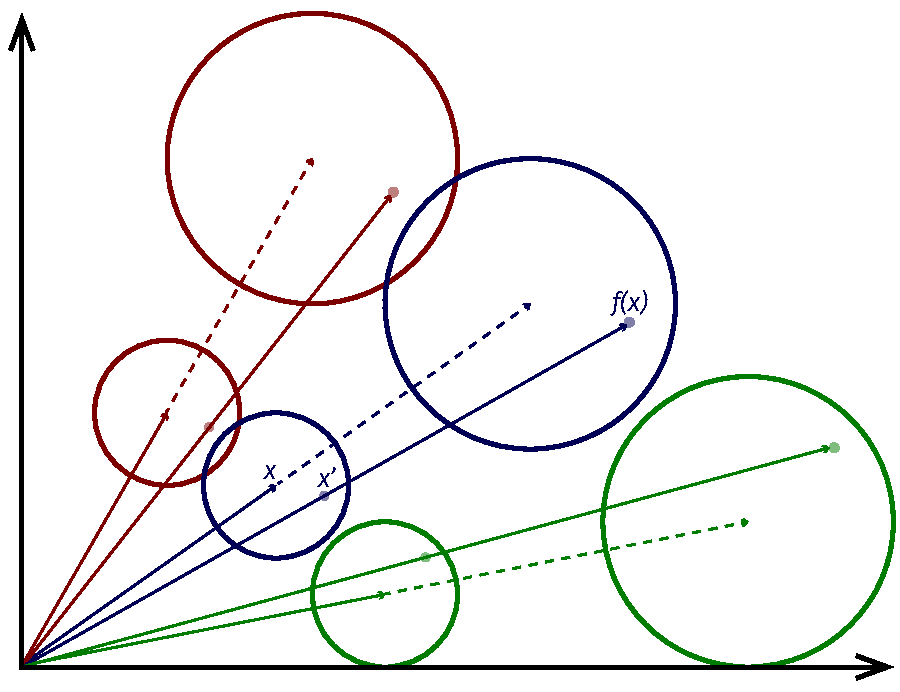
\includegraphics[width=0.5\columnwidth]{dcpe}
			\caption{Distance Comparison Preserving Encryption scheme \cite{dcpe}}%
		\end{figure}

	\end{frame}

	\begin{frame}{Search accuracy and TREC dataset}

		\begin{itemize}
			\item<1->
				Setup and query protocols: for given $\beta$
				\begin{itemize}
					\item Generate encryption key
					\item Encrypt dataset and queries set with $\beta$
					\item Run queries using conventional nearest-neighbor search (e.g., FAISS \cite{faiss})
					\item Report search accuracy metrics
				\end{itemize}

			\item<2->
				TREC 2020 dataset is 8.8M documents embedded with fine-tuned BERT \cite{bert} (768 dimensions) \\
				\begin{small}
					Thanks Hamed Zamani for the dataset
				\end{small}

			\item<3->
				Query is a 768-dimensional embedding asking for $k = \num{1000}$ closest documents \\
				\begin{small}
					TREC has set of documents, set of topics (questions), and relevance judgments (right answers)
				\end{small}

			\item<4->
				We report result set distance and difference, and ranking quality Recall, MRR and nDCG \\
				\begin{small}
					Set distance and difference measure pure \knn{} accuracy \\
					Recall, MRR and nDCG report ranking quality using relevance, common in informal retrieval literature
				\end{small}

		\end{itemize}

	\end{frame}

	\begin{frame}{Search accuracy results}

		\begin{figure}[h]
			\centering
			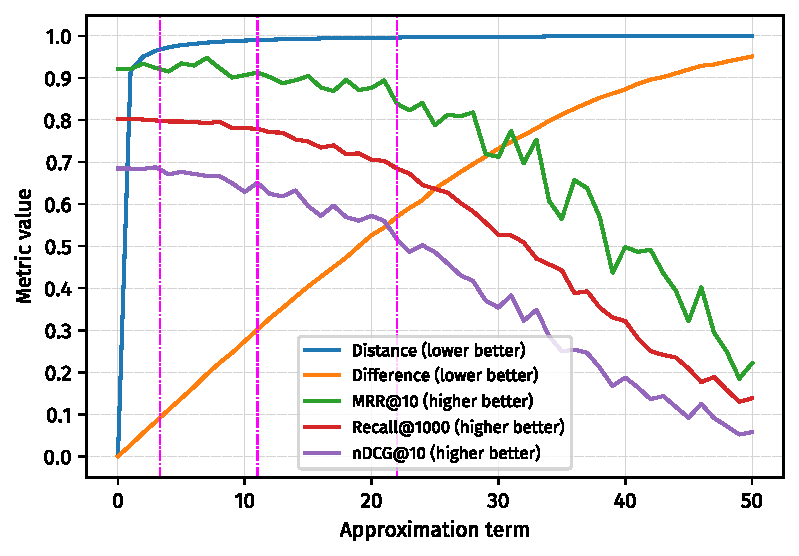
\includegraphics[width=0.7\textwidth]{knn-search}
			\caption{Rank quality metrics, result set distance and difference for $\beta \in \{ 0, 1, \ldots , 50 \} $}
		\end{figure}

	\end{frame}
